%% introPI.tex
%%
%% Presentation of the course ``Legal Issues'' of the Official Master on Libre Software (URJC)
%% http://master.libresoft.es
%%

%%---------------------------------------------------------------------
%%---------------------------------------------------------------------

\begin{frame}
  \frametitle{Course Contents}

%  \begin{itemize}[<+->]
  \begin{itemize}
    \item Lesson 0: Presentation of the Course
    \item \alert{Lesson 1: Intellectual Property: basic concepts and legal framework}
    \item Lesson 2: Legal Aspects of Libre Software
    \item Lesson 3: Libre software licenses
    \item Lesson 4: Free licenses for other intellectual works
    \item Lesson 5: Case studies
  \end{itemize}

\end{frame}


%%%%%%%%%%%%%%%%%%%%%%%%%%%%%%%%%%%%%%%%%%%%%%%%%%%%%%%%%%%%%%%%%%%%%%%
\section{Lesson I: Intellectual Property: basic concepts and legal framework}
%%%%%%%%%%%%%%%%%%%%%%%%%%%%%%%%%%%%%%%%%%%%%%%%%%%%%%%%%%%%%%%%%%%%%%%



%%---------------------------------------------------------------




%%%%%%%%%%%%%%%%%%%%%%%%%%%%%%%%%%%%%%%%%%%%%%%%%%%%%%%%%%%%%%%%%%%%%%%

\begin{frame}
\frametitle{The importance of licenses}
\textit{``\alert{I} \alert{A}m \alert{N}ot \alert{A} \alert{L}awyer (IANAL) and I never read licenses... why should I care about licenses?''}

\pause

\begin{itemize}[<+->]
\item Licenses provides terms of use of a work.
\item Licenses enable the opportunity to free a work.
\item Free licenses are not just another license: they are a declaration of principles, a social contract.
\end{itemize}
\bigskip

\pause

\alert{Licenses (free or not) are based on every country's \textit{copyright} law.}

\end{frame}

%%%%%%%%%%%%%%%%%%%%%%%%%%%%%%%%%%%%%%%%%%%%%%%%%%%%%%%%%%%%%%%%%%%%%%%


\begin{frame}
\frametitle{Law and Code}

\begin{itemize}
\item Tiny SCO group sued the huge IBM in 2005 put forward a cluster of complaints: trademarks, copyright infringements and theft of trade secrets...
\item Software patents lawsuits. 
\end{itemize}

\end{frame}




%%%%%%%%%%%%%%%%%%%%%%%%%%%%%%%%%%%%%%%%%%%%%%%%%%%%%%%%%%%%%%%%%%%%%%%

\subsection{What is Intellectual Property?}
\begin{frame}
\frametitle{What is Intellectual Property?}

\begin{itemize}
\item Intellectual Property (IP) refers to creations of the human mind.
\item IP is divided into two main categories: \alert{Industrial Property} (patents, trademarks) and \alert{Copyrights}.  

\vspace{1cm}

\begin{center}
{\large \alert{Patents}} \hspace{1.2cm}	{\LARGE \alert{Copyrights}} \hspace{1.2cm} 
{\large \alert{Trademarks}}
\end{center}

\end{itemize}

\end{frame}

%%%%%%%%%%%%%%%%%%%%%%%%%%%%%%%%%%%%%%%%%%%%%%%%%%%%%%%%%%%%%%%%%%%%%%%
\subsection{IP Definitions}
\begin{frame}
\frametitle{IP: Concepts}

\begin{itemize}
\item I'is a broad concept that covers several types of legally recognized rights.
\item IP rights are rights to \alert{intangible things} (``ideas'').
	\begin{itemize}
	\item as expressed (``copyrights''), 
	\item or as em­bodied in a practical implementation (``patents'')
	\end{itemize}
\item In today’s legal systems, IP (including Industrial Property) typically includes at least \alert{copy­rights}, \alert{trademarks}, \alert{patents}, and \alert{trade secrets}.

\end{itemize}

\end{frame}


%%%%%%%%%%%%%%%%%%%%%%%%%%%%%%%%%%%%%%%%%%%%%%%%%%%%%%%%%%%%%%%%%%%%%%%

\begin{frame}
\frametitle{Intellectual Property: WIPO Definition}

\textsc{WIPO} gives an ``common law'' definition of IP:

\begin{block}{WIPO Definition}
  Intellectual property refers to creations of the mind:
  inventions, literary and artistic works, and symbols, names, images,
  and designs used in commerce.
\end{block}

\end{frame}

%%%%%%%%%%%%%%%%%%%%%%%%%%%%%%%%%%%%%%%%%%%%%%%%%%%%%%%%%%%%%%%%%%%%%%%

\begin{frame}
\frametitle{Origins}

\begin{itemize}
\item With the invention of the printing press ($\sim$1450), works became commercial objects.
\item First forms of plagiarism appeared, so that editors forced legislators
to regulate and protect the original works.
\item Regulation was also conceived as a way of controlling information (i.e.
censorship)
\end{itemize}

\end{frame}

%%%%%%%%%%%%%%%%%%%%%%%%%%%%%%%%%%%%%%%%%%%%%%%%%%%%%%%%%%%%%%%%%%%%%%%

\begin{frame}
\frametitle{Pro-IP Arguments}

\begin{itemize}
\item \alert{Utilitarian Defense of IP}: Laws and policies that maximize  ``wealth'' or ``utility'' (Common Law)
\item \alert{Natural-Rights arguments}: creations of the mind are entitled to protection just as tan­gible property is. (Continental Law)
\end{itemize}

\end{frame}

%%%%%%%%%%%%%%%%%%%%%%%%%%%%%%%%%%%%%%%%%%%%%%%%%%%%%%%%%%%%%%%%%%%%%%%

\begin{frame}
\frametitle{IP Criticism}

\begin{itemize}
\item A long tradition of opposition to patent and copyrights.
\item Econometric studies don't conclusively show net gains in wealth.
\item Costs of the patent system.
\item Ethical issues: more innovation and creativ­ity wouldn't justify restricting the free­dom of individuals to use their physical property.
\item It's not coherent: protects only certain types of creations.
\item Distinction between creation and discovery is not clear­cut or rigorous.
\item Creations of the mind are not as tan­gible property is.
\end{itemize}

\end{frame}


%%%%%%%%%%%%%%%%%%%%%%%%%%%%%%%%%%%%%%%%%%%%%%%%%%%%%%%%%%%%%%%%%%%%%%%
\subsection{Intellectual Property vs Tangible Property}
\begin{frame}
\frametitle{Intellectual Property vs Tangible Property}

\begin{center}
\Large
What are the differences?
\end{center}

\end{frame}

%%%%%%%%%%%%%%%%%%%%%%%%%%%%%%%%%%%%%%%%%%%%%%%%%%%%%%%%%%%%%%%%%%%%%%%


\begin{frame}
\frametitle{Types of Property}


\begin{itemize}
\item \alert{Immovable property} (realty, land, houses...) 
\item \alert{Moveable property} (chairs, cars, clocks...).
\end{itemize}
\pause
\begin{center}
\alert{Tangible rights}
\end{center}
\pause
\medskip

Property attributes:
\pause
\begin {itemize}
\item \alert{Antagonistic} (if I take your car, you don't have one yet)
\pause
\item \alert{Excludable} (You close your car, I can't enter)
\pause
\item \alert{Scarcity} (conflict over resources)
\end{itemize}


\end{frame}

%%%%%%%%%%%%%%%%%%%%%%%%%%%%%%%%%%%%%%%%%%%%%%%%%%%%%%%%%%%%%%%%%%%%%%%

\begin{frame}
\frametitle{IP vs. tangible property}

\begin{quote}
\footnotesize{''If you have an apple and I have an apple and we exchange these apples then you and I will still each have one apple. But if you have an idea and I have an idea and we exchange these ideas, then each of us will have two ideas.''} \textsc{George Bernard Shaw} (1856-1925)
\end{quote}

\pause

\begin {itemize}
\item Not antagonistic (if I take your idea, you still maintain it) 
\item Not excludable (Your use does not exclude my use)
\item Not scarcity (ideas are not scarce)
\end{itemize}
\begin{center}
Intellectual Property: \alert{Intangible rights} \\
\pause
\textbf{oxymoron?}
\end{center}
\end{frame}

%%%%%%%%%%%%%%%%%%%%%%%%%%%%%%%%%%%%%%%%%%%%%%%%%%%%%%%%%%%%%%%%%%%%%%%

\begin{frame}
\frametitle{IP vs. physical property}

More differences between Intellectual Property and Tangible (``physical'')
Property:
\begin{itemize}
\item Expiration date.
\item When you copy the IP resource, you don't harm to the owner of
  copied object. However, a copy can harm the author.
\item it is difficult to see the difference between ``copy'' (plagiarism) and
``inspiration''. 
\end{itemize}

\end{frame}



%%%%%%%%%%%%%%%%%%%%%%%%%%%%%%%%%%%%%%%%%%%%%%%%%%%%%%%%%%%%%%%%%%%%%%%

\begin{frame}
\frametitle{IP Categories (Continental Law)}

IP is divided into two categories (Continental Law):  

\begin{itemize}
\item \alert{Industrial property}: inventions, patents, trademarks, industrial designs, and geographic indications of source. 
\item \alert{Copyright} (''Author's Rights''): literary and artistic works such as novels, poems and plays, films, musical works, artistic works such as drawings, paintings, photographs and sculptures, and architectural designs.  
\end{itemize}

Rights related to copyright include those of performing artists in their performances (``neighboring rights'').  

\end{frame}


%%%%%%%%%%%%%%%%%%%%%%%%%%%%%%%%%%%%%%%%%%%%%%%%%%%%%%%%%%%%%%%%%%%%%%%
\subsection{Types of IP}
\begin{frame}
\frametitle{IP Types (Common Law)}

\alert{Common law} system:
\begin{itemize}
\item \alert{Copyrights}: Protect from unauthorized copy: artistic or literary
  works, computer programs, data collections, industrial designs, etc.
\item \alert{Trademarks}: Protect company symbols and names.
\item \alert{Trade secrets}: Protect access to some industrial secrets.
\item \alert{Patents}: Protect the rights of exploiting inventions as monopolies.
\end{itemize}

\end{frame}



%%%%%%%%%%%%%%%%%%%%%%%%%%%%%%%%%%%%%%%%%%%%%%%%%%%%%%%%%%%%%%%%%%%%%%%


\begin{frame}
\frametitle{Trade secrets}

\begin{itemize}
\item A trade secret is a way to protect investments in industrial area,
through Industrial Property laws.
\item Under trade secrets, there are several goods such as chemical or pharmaceutical
formulas, but also software.
\item An example would be the formula for Coca-cola
\item Proprietary software enterprises hide the source code of their
software products as a way to protect their investment in creating
such software.
\item Trade secret protection is obtained by declaring that the details
of a subject are secret.
\item However, disclosure, reverse-engineering, or independent in­vention may destroy it.
\end{itemize}

\end{frame}

%%%%%%%%%%%%%%%%%%%%%%%%%%%%%%%%%%%%%%%%%%%%%%%%%%%%%%%%%%%%%%%%%%%%%%%

\begin{frame}
\frametitle{Why Trade secrets?}

\begin{center}
\textbf{Why trade secret protection instead of patents?}
\end{center}

\pause

\begin{itemize}
\item it's not novel enough to be subject to patent protection, 
\item or not original enough to be protected by copyright.
\end{itemize}

\end{frame}


%%%%%%%%%%%%%%%%%%%%%%%%%%%%%%%%%%%%%%%%%%%%%%%%%%%%%%%%%%%%%%%%%%%%%%%

\begin{frame}
\frametitle{Trademarks}

\begin{itemize}
\item It's a word, phrase, symbol, or design used to identify
the source of goods or services sold, and to distinguish them from the
goods or services of others. 
\item Related to trademark protection: rights against forms of cybersquatting, 
and various ``unfair competition'' claims.
\end{itemize}

\end{frame}

%%%%%%%%%%%%%%%%%%%%%%%%%%%%%%%%%%%%%%%%%%%%%%%%%%%%%%%%%%%%%%%%%%%%%%%

\begin{frame}
\frametitle{Trademarks (2)}

\begin{itemize}
\item Sometimes, the names are not registered in most countries and this
implied some problems. {\small For example, in USA somebody registered the
trademark ``Linux'' and tried to obtain money for its use.}
\item In FLOSS world, not very important, probably because
registering a trademark is not free and most developers do not pay
attention on them. 
\item However, there are some well known trademarks in
this world, such as GNOME, GNU, Debian.
\end{itemize}

\end{frame}



%%%%%%%%%%%%%%%%%%%%%%%%%%%%%%%%%%%%%%%%%%%%%%%%%%%%%%%%%%%%%%%%%%%%%%%

\begin{frame}
\frametitle{Patents}

\begin{itemize}
\item A patent is a property right in \alert{inventions}, that is, in devices or
processes that perform a ``useful'' function.
\item A patent grants the inventor a limited \alert{monopoly} (20 years) on the
manufacture, use, or sale of the invention. 
\item The invention is not protected by secret. On the contrary, the
  invention is publicly available.
\item For exploiting the invention the interested company must pay a license.
\item A patent actu­ally only grants to the patentee the right \alert{to exclude} (i.e., to prevent others from practicing the patented invention). Why?
\end{itemize}

\end{frame}

%%%%%%%%%%%%%%%%%%%%%%%%%%%%%%%%%%%%%%%%%%%%%%%%%%%%%%%%%%%%%%%%%%%%%%%

\begin{frame}
\frametitle{Patents (2)}

\begin{itemize}

\item Patents can be obtained only for ``practical applications'' of ideas.
\item Not for more abstract or theoretical ideas.
\item Philosophical, mathematical or scientific truths cannot be protected. (Why?)
\item Christmas Tree Stand Watering System (US Patent)
\item Einstein’s ``discovery'' of the relation $E=mc^2$ is unpantentable.
\item Distinction between \alert{creation} (patentable) and \alert{discovery} (unpatentable) is not clear­.
\end{itemize}

\end{frame}


%%%%%%%%%%%%%%%%%%%%%%%%%%%%%%%%%%%%%%%%%%%%%%%%%%%%%%%%%%%%%%%%%%%%%%%

\begin{frame}
\frametitle{Patents. Debate}

\begin{itemize}
\item Is it fair to reward more \alert{practical inventors} and entertainment providers (engineers and song­writers), and to leave more \alert{theoretical science} and \alert{math researchers} and \alert{philosophers} unrewarded?


\end{itemize}

\end{frame}



%%%%%%%%%%%%%%%%%%%%%%%%%%%%%%%%%%%%%%%%%%%%%%%%%%%%%%%%%%%%%%%%%%%%%%%
\subsection{Legal Framework}

\begin{frame}
\frametitle{IP: Legal Framework}

IP Laws are coordinated in nearly all the world, thanks to several
organizations and initiatives:

\begin{columns}

\column[t]{2.5cm}

\begin{figure}
\vspace{-0.6cm}
\begin{flushleft}
	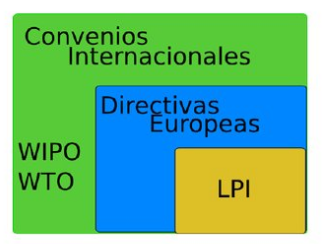
\includegraphics[scale=0.3,clip=true]{figs/legal_framework.png}
\end{flushleft}
\end{figure}


\column[t]{8cm}

\begin{itemize}
\item WIPO: Promotes both property types.
\item TRIPS: Establishes minimal conditions to all countries of WTO.
\item International agreements: Bern and Geneva Convention. 
\end{itemize}

\end{columns}

\small
\begin{block}{Universal Declaration on Human Rights, art. 27.2}
Everyone has the right to the protection of the moral and material interests resulting from any scientific, literary or artistic production of which he is the author.
\end{block}


\end{frame}


%%%%%%%%%%%%%%%%%%%%%%%%%%%%%%%%%%%%%%%%%%%%%%%%%%%%%%%%%%%%%%%%%%%%%%%

\begin{frame}
\frametitle{Spanish Legal framework}

\begin{itemize}
\item Ley de Propiedad Intelectual (LPI): Continental law. 
\item Derechos de autor vs. Derechos afines (o ` conexos'' , or ``vecinos'') 
\item Derechos morales vs. Derechos de explotación (``patrimoniales'')
\end{itemize}

\end{frame}


%%%%%%%%%%%%%%%%%%%%%%%%%%%%%%%%%%%%%%%%%%%%%%%%%%%%%%%%%%%%%%%%%%%%%%%

\begin{frame}
\frametitle{IP: Works protected}

The type of works considered include:

\begin{itemize}
\item Literature works (novels, poems, theater works, reference documents, newspapers and software)
\item Artistic works 
\item Scientific works 
\item Databases, movies 
\item Musical compositions and choreographies, architectonic works, publicity 
\item Maps and technical paintings
\end{itemize}

\begin{center}
\footnotesize
Like literature and music, \alert{software} is protected primarily by copyright law: \\ It is a \alert{literary work}.
\end{center}

\end{frame}


%%%%%%%%%%%%%%%%%%%%%%%%%%%%%%%%%%%%%%%%%%%%%%%%%%%%%%%%%%%%%%%%%%%%%%%

\begin{frame}
\frametitle{Authors and copyright holders}

\begin{itemize}

\item Authors is a (physical or juridical) person that creates
a work. 

\item \alert{Collaborative work}: unitary result of the collaboration
of several authors where the input of each author may be
identified and exploit independently.
\item \alert{Collective work} (art. 8 LPI): under the initiative and coordination of
a physical or juridical person. It groups the input
of several authors that cannot be identified independently
and that compose a unique and autonomous creation. {\footnotesize Examples: GNOME,
Mozilla, FSF, etc.}
\item Usually IP rights are transferred to enterprises where creators
work (for example, the companies where the programmers work). 
\item But the moral rights are still retained by the programmer.


\end{itemize}

\end{frame}


%%%%%%%%%%%%%%%%%%%%%%%%%%%%%%%%%%%%%%%%%%%%%%%%%%%%%%%%%%%%%%%%%%%%%%%

%\begin{frame}
%\frametitle{The Copyright: Protection for Authors}
%
%Copyright, a set of exclusive rights:
%\begin{itemize}
%\item To regulate the use of a particular expression of an idea or
%  information.
%\item In most cases, with limited duration.
%\end{itemize}
%
%The copyright is granted to all intellectual publications without any other
%requirements:
%\begin{itemize}
%\item Automatic copyright when the work is published.
%\item (Almost) global scope.
%\end{itemize}
%
%\end{frame}

%%%%%%%%%%%%%%%%%%%%%%%%%%%%%%%%%%%%%%%%%%%%%%%%%%%%%%%%%%%%%%%%%%%%%%%

\begin{frame}
\frametitle{The Copyright: Protection for Authors}

The rights protected by copyright laws:
\begin{itemize}
\item \alert{Moral rights}. Guarantee work dissemination and author attribution.
Only in Continental law.
\item \alert{Economic rights} (\textbf{copyright} \textit{per se} in Common Law). Property rights, guarantee economic exploitation.
\end{itemize}


\end{frame}

%%%%%%%%%%%%%%%%%%%%%%%%%%%%%%%%%%%%%%%%%%%%%%%%%%%%%%%%%%%%%%%%%%%%%%%

\begin{frame}
\frametitle{The Copyright Term}

Copyright expires after:

\begin{itemize}
\item Minimum: 50 years after death of person. 
\item In general (USA, Europe): 70 years after \textit{post mortem}.
\item When its term expires, a work goes into Public Domain.
\end{itemize}
\pause
\begin{center}
Automatic copyright when the work is published.
\end{center}

\end{frame}


%%%%%%%%%%%%%%%%%%%%%%%%%%%%%%%%%%%%%%%%%%%%%%%%%%%%%%%%%%%%%%%%%%%%%%%

\begin{frame}
\frametitle{Moral rights}

\begin{itemize}
\item Disclosure of the work
\item Way of publication: with his name, a pseudonym or anonymously
\item The right of attribution
\item The right to the integrity of the work (distortion or mutilation)
\item The withdrawal of his work (addressing compensation if needed)
\end{itemize}

\end{frame}

%%%%%%%%%%%%%%%%%%%%%%%%%%%%%%%%%%%%%%%%%%%%%%%%%%%%%%%%%%%%%%%%%%%%%%%

\begin{frame}
\frametitle{Moral rights (2)}

\begin{itemize}
\item These rights cannot be withdrawn, cannot be transferred, are inalienable
and some even perpetual.
\item Included in the Bern Convention in 1928. 
\item The US do not completely recognize moral rights as part of copyright law, but rather as part of other bodies of law, such as defamation, academic fraud or unfair competition (plagiarism).
\end{itemize}


\end{frame}


%%%%%%%%%%%%%%%%%%%%%%%%%%%%%%%%%%%%%%%%%%%%%%%%%%%%%%%%%%%%%%%%%%%%%%%

\begin{frame}
\frametitle{Economic rights (copyright)}

\begin{itemize}
\item \alert{Reproduction} (includes communication and copying): loading,
presentation on the screen, execution, transmission and storage.
\begin{itemize}
\item Even for using a program you require the author's approval!
\item The right to copy/reproduce is fundamental in licenses; else
the software cannot be run.
\item Stealing a book: attempting against the owner
of the book but not the owner of the IP. 
\end{itemize}
\item \alert{Distribution:} Public disposal of physical copies {\small(i.e. offering
the software over the Internet is not included). Software is not
sold as this could make re-selling possible. What is sold is the CD; the
software is licensed!}
\item \alert{Public performance:} there is no distribution of physical copies {\small(What is public and private on the Internet?)}
\item \alert{Transformation} {\small(for instance, translation)}
\end{itemize}


\end{frame}

%%%%%%%%%%%%%%%%%%%%%%%%%%%%%%%%%%%%%%%%%%%%%%%%%%%%%%%%%%%%%%%%%%%%%%%

\begin{frame}
\frametitle{Copyright in short}

Gives its owner an ``exclusive right'' to:

\begin{itemize}
\item To make and sell copies of the work (including,
typically, electronic copies).
\item To make derivative works
\item to publicly perform/display the work
\item To sell or assign these rights to others
\end{itemize}

\end{frame}


%%%%%%%%%%%%%%%%%%%%%%%%%%%%%%%%%%%%%%%%%%%%%%%%%%%%%%%%%%%%%%%%%%%%%%%

\begin{frame}
\frametitle{Copyright in short}

\begin{itemize}
\item Limitation on the \alert{expression} of an idea (it's possible another expressions of the same idea).
\item Gives exclusive rights to the owner.
\item Economic rights have time expiration.
\item There are exceptions (fair use)
\item By default, all rights reserved.
\item In software the expression is given by the code; algorithms are
not protected.
\item There are neighboring rights.

\end{itemize}

\end{frame}



%%---------------------------------------------------------------
%%%%%%%%%%%%%%%%%%%%%%%%%%%%%%%%%%%%%%%%%%%%%%%%%%%%%%%%%%%%%%%%%%%%%%%
% \section{References}
%%%%%%%%%%%%%%%%%%%%%%%%%%%%%%%%%%%%%%%%%%%%%%%%%%%%%%%%%%%%%%%%%%%%%%%

\begin{frame}
\frametitle{References}

\begin{itemize}
\item \textsc{Van Lindberg}, \textit{Intellectual Property and Open Source}, O'Reilly, July 2008.
\item \textsc{Malcolm Bain} et al. \textit{Aspectos legales y de explotación del software libre}, UOC, February 2007. \\
{\footnotesize \url{http://ocw.uoc.edu/informatica-tecnologia-y-multimedia/aspectos-legales-y-de-explotacion-del-software-libre/materiales/}}
\item \textsc{Lawrence Rose}, \textit{Open Source Licensing}, Prentice Hall, July 2004 
% \item Text for CC Attribution-ShareAlike 3.0 License \\ 
% \url{http://creativecommons.org/licenses/by-nc-sa/3.0/legalcode}

\end{itemize}

\end{frame}

%%%%%%%%%%%%%%%%%%%%%%%%%%%%%%%%%%%%%%%%%%%%%%%%%%%%%%%%%%%%%%%%%%%%%%%




